\documentclass{../template/Report}%方括号内写yuxi即生成预习报告
\settemplatedir{../template/}%设置模板路径

\exname{} %实验名称
\extable{} %实验桌号
\instructor{} %指导教师
\class{} %班级
\name{} %姓名
\stuid{} %学号

\nyear{} %年
\nmonth{} %月
\nday{} %日
\nweekday{} %星期几
\daypart{}%上午/下午

\redate{} %如有实验补做，补做日期
\resitu{} %情况说明：

\begin{document}
\maketitle

\section{预习报告}
\subsection{实验综述}

\subsubsection{自组惠斯登电桥测量未知电阻}
本实验采用自组惠斯登电桥电路进行测量，电路结构如\cref{huisideng}所示。电路中包含两个比例臂电阻 $R_1, R_2$，一个待测电阻 $R_x$ 以及一个比较臂电阻 $R_s$。实验操作时，需调节可变电阻 $R_s$ 的阻值，使得检流计 $G$ 指向零位，此时电桥达到平衡状态（即 $B、D$ 两点电势相等）。根据电桥平衡原理，满足 $I_1R_1=I_2R_2$ 及 $I_1R_x=I_2R_s$，由此导出待测电阻计算式：
\[
    R_x = \frac{R_1}{R_2} R_s
\]
式中 $\frac{R_1}{R_2}$ 定义为电桥的比率。为了保证测量精度，实验中需要合理选择倍率，确保读数具有4位有效数字。

为了消除比例臂电阻 $R_1, R_2$ 本身误差带来的影响，本实验采用“交换法”：保持其他条件不变，交换 $R_x$ 与 $R_s$ 的位置重新进行平衡调节，得到新的阻值 $R_s'$。最终待测电阻值取两次测量的几何平均值：$\overline{R_x} = \sqrt{R_sR_s'}$。

\begin{figure}[H]
    \centering
    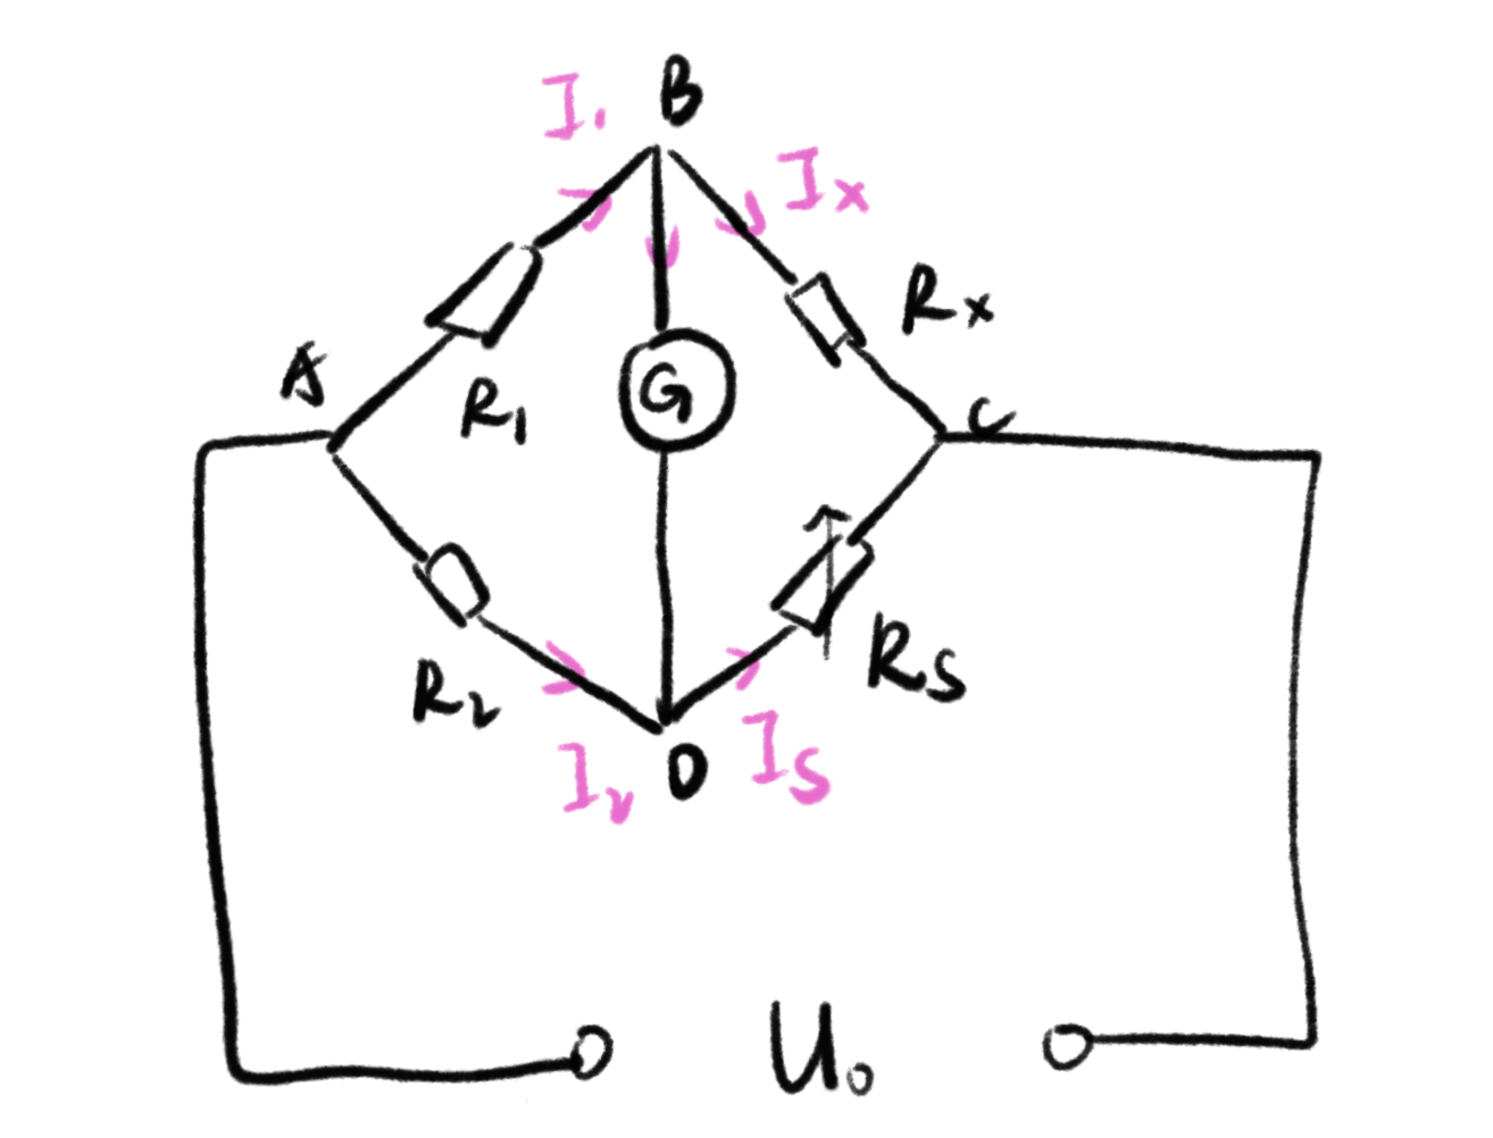
\includegraphics[width=0.4\textwidth]{figures/5/电路.pdf}
    \caption{惠斯登电桥原理图}
    \label{huisideng}
\end{figure}

关于实验误差分析，主要考虑两部分来源：电阻箱 $R_s$ 的仪器误差以及检流计灵敏度引入的读数误差。
首先，电阻箱引入的相对误差计算如下：
\[\frac{\Delta R_x}{R_x} \approx \frac{\Delta R_s}{R_s}\]
对于实验室常用的 0.1 级十进位直流电阻箱，其允许误差由精度等级 $a$（通常为0.1）和残余电阻系数 $b$（通常为0.2）决定，总盘数为 $m$。则电阻箱的极限误差为：
\[\Delta R_s = \pm (0.001 R_s + 0.002 m)\]

其次，需考虑电桥灵敏度带来的误差。电桥灵敏度 $S$ 定义为单位相对电阻变化引起的检流计偏转格数：
\[S = \frac{\Delta d}{\Delta R_s /R_s}\]
实验中需要实测 $S$ 值。假设人眼能分辨的检流计最小偏转为 0.2 格（$\Delta d = 0.2$），则由灵敏度限制导致的相对误差为：
\[\frac{\Delta R_{s\text{检}}}{R_{s\text{检}}} = \frac{0.2}{S}\]

综合上述两项，待测电阻的总相对不确定度合成公式为：
\[E = \frac{\Delta R_x}{\overline{R_x}} = \sqrt{\left(0.001+ \frac{0.002m}{R_s}\right)^2 + \left(\frac{0.2}{S}\right)^2}\]

最终的绝对不确定度为 $u = \Delta R_x = E \overline{R_x}$，测量结果记为：
\[R_x = \overline{R_x} \pm \Delta R_x\]

\textbf{需记录与处理的数据}：倍率设定值 $\frac{R_1}{R_2}$、交换前后的电阻箱读数 $R_s$ 与 $R'_s$、灵敏度测定相关数据，以及最终计算出的相对误差 $E$、不确定度 $u$ 和电阻结果 $R_x$。

\subsubsection{使用QJ\_23型箱式电桥测定电阻离散度}
本部分使用封装好的 QJ\_23 型箱式电桥。连接电源并调零后，对接线盘上的 8 个标称值相同的电阻依次进行测量。测量时需注意选择合适的倍率旋钮，保证读数有足够的有效数字。

实验目标是计算这组电阻的离散度，公式为 $\frac{S}{\overline{R_x}} \times 100\%$。

\textbf{需记录与处理的数据}：8 个电阻的测量原始数据、计算出的平均值、标准差及离散度百分比。

\subsection{实验重点}
\begin{enumerate}
    \item 熟悉惠斯登电桥的平衡原理，能够独立搭建电桥电路测电阻；
    \item 学习并应用不确定度的评定方法，掌握误差合成的技巧；
    \item 熟悉 QJ\_23 型箱式电桥的操作规范；
    \item 学会运用贝塞尔公式处理数据，计算标准差与离散度。
\end{enumerate}

\subsection{实验难点}
\begin{enumerate}
    \item 实际电路的搭建与调试，特别是排除接触不良等故障；
    \item 深入理解电桥灵敏度对测量精度的影响；
    \item 繁琐的数据处理过程，特别是误差公式的准确代入与计算；
    \item 对标准差、离散度等统计学概念的理解与计算。
\end{enumerate}

\begin{fullreportonly}
    \section{结果与分析}
    \subsection{数据处理与结果}
    \subsubsection{交换法测量未知电阻}

    实验首先采用交换法对未知电阻进行测量。为了保证测量精度，比率臂电阻选取为 $R_1=R_2 = 1000 \si{\ohm}$，使得倍率为1。

    在交换待测电阻前后，分别调节电阻箱平衡，测得阻值分别为 $R_s = \SI{224.6}{\ohm}$ 和 $R'_s = \SI{224.5}{\ohm}$。根据交换法原理，待测电阻的阻值应为两次测量的几何平均值：
    \[\overline{R_x} = \sqrt{R_s R'_s} = \sqrt{224.6 \times 224.5} \approx \SI{224.5}{\ohm}\]

    随后对电桥灵敏度进行了测定。保持 $R_s$ 在 $\SI{224.5}{\ohm}$ 附近，将阻值改变 $\Delta R_s = \SI{0.3}{\ohm}$，观察到检流计指针偏转了 $\Delta d = 29$ 格。

    计算电桥灵敏度时，考虑到 $\Delta R_s = 0.3$ 仅有一位有效数字，根据有效数字运算规则，结果也应保留一位：
    \[S = \frac{\Delta d}{\frac{\Delta R_s}{R_s}} = \frac{29}{\frac{0.3}{224.6}} \approx 2 \times 10^4\]

    根据公式，计算 $R_x$ 的相对不确定度：
    \[E = \frac{\Delta R_x}{\overline{R_x}} = \sqrt{\left(0.001+ \frac{0.002}{R_s}\right)^2 + \left(\frac{0.2}{S}\right)^2} \approx 0.10\% \]

    由此得到绝对不确定度 $\Delta R_x = E \cdot \overline{R_x} \approx \SI{0.2}{\ohm}$。
    最终测量结果表示为：
    \[R_x = (\overline{R_x} \pm \Delta R_x) = (224.5 \pm 0.2)\,\si{\ohm}\]

    \subsubsection{用QJ\_23型盒式惠斯登电桥测电阻离散度}

    实验选取 $0.1$ 倍率，对给定的八个待测电阻进行直接测量，记录数据如\cref{yiduidianzu}所示。

    \begin{table}[H]
        \caption{电阻离散度测量数据}
        \centering
        \begin{tabular}{C{0.1\textwidth}C{0.08\textwidth}C{0.08\textwidth}C{0.08\textwidth}C{0.08\textwidth}C{0.08\textwidth}C{0.08\textwidth}C{0.08\textwidth}C{0.08\textwidth}}
            \toprule
            编号             & 1     & 2     & 3     & 4     & 5     & 6     & 7     & 8     \\
            \midrule
            阻值/$\si{\ohm}$ & 681.2 & 680.4 & 676.6 & 681.9 & 683.0 & 680.8 & 688.8 & 677.2 \\
            \bottomrule
        \end{tabular}
        \label{yiduidianzu}
    \end{table}

    通过计算可知，这组电阻的平均值为 $\overline{R} = \SI{681.2}{\ohm}$。
    计算标准偏差：
    \[S_{dev} = \sqrt{\frac{\sum(R_{i} - \overline{R})^2}{n-1}} \approx \SI{3.8}{\ohm}\]

    这批电阻的离散度为：
    \[\frac{S_{dev}}{\overline{R}} \times 100\% = \frac{3.8}{681.2} \times 100\% \approx 0.56\% \]

    相对误差（与标称值 $\SI{680}{\ohm}$ 比较）：
    \[ \eta_2 = \frac{|\overline{R} - 680|}{680} \times 100\% = \frac{|681.2 - 680|}{680} \times 100\% \approx 0.18\% \]

    \subsection{误差分析}
    \subsubsection{相对误差计算}
    已知待测电阻的标准值为 $R_{std} = \SI{220}{\ohm}$，本次实验测得的平均值为 $\overline{R_x} = \SI{224.6}{\ohm}$。
    则相对误差为：
    \[ \eta = \frac{|\overline{R_x} - R_{std}|}{R_{std}} \times 100\% = \frac{|224.6 - 220|}{220} \times 100\% \approx 2.09\% \]
    可以看到测量值比标准值偏大，约为 $2\%$ 的偏差。

    \subsubsection{误差来源分析}
    交换法测量未知电阻：
    \begin{enumerate}
        \item \textbf{电源电压与检流计灵敏度的匹配问题：}
              \begin{itemize}
                  \item 在实验调试过程中，我发现单纯追求高灵敏度并不可行。起初我尝试将电源电压调至最大，并将其灵敏度调至较低档，结果发现电桥整体灵敏度 $S$ 不足，导致无法分辨微小的电阻变化；
                  \item 随后我尝试减小电源电压，同时将检流计灵敏度调高一档。虽然理论上灵敏度够了，但在实际操作中，检流计指针变得极不稳定，受环境干扰严重，导致无法准确判断零点，难以调整平衡。
                  \item 这说明电桥测量的首要条件是保证电桥能稳定平衡。盲目提高检流计档位会引入噪声，反而增大了读数的人为误差。
              \end{itemize}

        \item \textbf{电阻本身的误差：}
              实验室使用的电阻可能与标称值之间存在误差。

        \item \textbf{电流热效应的影响：}
              测量结果 $\SI{224.6}{\ohm}$ 明显高于标准值 $\SI{220}{\ohm}$。电流流过待测电阻产生的焦耳热可能导致电阻温度升高。对于金属导体，电阻随温度升高而增大，可能会引入正向的偏差。

        \item \textbf{电阻箱与连接误差：}
              虽然使用了交换法消除比率臂的不等臂误差，但电阻箱本身的示数误差无法消除。此外，导线接入点的接触电阻如果接触不良，也会串联进 $R_x$ 回路中，导致测量值偏大。

        \item \textbf{实际灵敏度不足导致的死区误差：}
              虽然计算出的灵敏度尚可，但在实际调节 $R_s$ 时，受限于电阻箱 $0.1$ 级的最小步进，检流计可能在 $0.1\Omega$ 的变化范围内都处于指针为0的假平衡状态，这部分无法分辨的阻值变化直接构成了偶然误差。
    \end{enumerate}

    测电阻离散度：
    在测量批量电阻时，虽然 $\overline{R} = \SI{681.2}{\ohm}$ 与标称值 $\SI{680}{\ohm}$ 较为接近，但个体的离散情况比较严重。
    从数据上看，最大的达到了 $\SI{688.8}{\ohm}$，最小的只有 $\SI{676.6}{\ohm}$，两者相差了 $\SI{12.2}{\ohm}$。
    这说明这批电阻的制造工艺一致性一般，或者因老化程度不同导致阻值出现了较大的随机分布。
    \subsection{实验探讨}

    这次用惠斯登电桥测电阻，最大的感受是“平衡”的思想在精密测量中的重要性。
    特别是使用了交换法后，明显感觉到这种方法巧妙地抵消了桥臂不对称带来的系统误差。
    虽然数据处理时计算稍微繁琐一点，但对有效数字的取舍和误差传递的理解比以前更深刻了。

    \section{思考题}

    \subsection{为什么用惠斯登电桥测电阻比伏安法测量的准确度高？用电桥法测电阻产生误差的主要因素是什么？}

    惠斯登电桥法相较于伏安法具有更高的准确度，在于测量原理的不同。
    伏安法属于偏转测量法，无论采用内接法还是外接法，电表的内阻都会接入电路，从而引入不可消除的系统误差。
    而惠斯登电桥法，当电桥处于平衡状态时，检流计支路电流为零（$I_g = 0$），此时电桥臂对电路无分流或分压效应，从理论上完全消除了电表内阻对测量结果的影响。

    然而，电桥法在实际操作中仍存在误差，
    主要来源包括：首先是标准电阻的不确定度，即比率臂和比较臂电阻箱本身的精度等级限制；
    其次是检流计灵敏度的限制，当电桥处于极微小的非平衡状态时，若电流未达到检流计的感应阈值，
    指针仍指示零位，这将产生死区误差；此外，导线接触点的接触电阻、热电势以及在大电流下电阻元件因自热效应引起的阻值漂移，均为产生误差的重要因素。

    \subsection{为了提高电桥测量灵敏度，应采取哪些措施？为什么？}

    电桥灵敏度 $S$ 定义为单位相对阻值变化引起的检流计偏转格数。为了提高测量灵敏度，通常采取以下措施：

    首要措施是适当提高电源电压，$S$ 与电源电压成正比。
    在不超出桥臂电阻额定功率的前提下，提高电压可增大回路电流，使得同样的电阻失衡产生更大的不平衡电压，从而驱动检流计偏转。
    其次是选用高灵敏度的检流计。检流计的电流常数越小，对微弱电流的响应越灵敏，从而能分辨更细微的电阻变化。
    此外，根据电路理论，当桥臂电阻数值尽量接近且检流计内阻与电桥输出电阻匹配时，电桥的灵敏度相对较高。

    \subsection{用电桥测电阻时，若线路接通后检流计指针总是往一个方向偏转或总不偏转，试分析是什么原因？}

    在实验过程中，若检流计状态异常，通常对应着特定的电路故障：

    若指针总是向一个方向偏转，这表明电桥始终处于严重的失衡状态，且无法通过调节 $R_s$ 达到平衡。主要原因可能是比率臂选择不当，导致待测电阻 $R_x$ 超出了比较臂电阻箱 $R_s$ 的调节范围；
    或者是电桥的某一桥臂出现了断路或短路故障，致使电位分布极不对称。

    若指针完全不偏转，则说明检流计支路无电流通过。
    这通常并非电桥达到平衡状态，而很有可能电路发生了开路。常见原因包括电源未接通、电源开关接触不良、导线内部断裂，或者是检流计本身线圈烧断或保险丝熔断。

    \subsection{惠斯登电桥比率臂选取的原则是什么？为什么要这样选取？}

    比率臂（即倍率 $K = R_1 / R_2$）的选取原则是：使比较臂电阻箱 $R_s$ 的读数尽可能大，充分利用其全部有效位数。

    这样选取的目的在于保证测量结果的有效数字位数，从而降低相对误差。
    例如，若待测电阻约为几百欧姆，若选倍率为 $1$，则 $R_s$ 读数仅为几百，有效数字可能只有3位；若选倍率为 $0.1$，
    则 $R_s$ 读数可达几千，有效数字可提升至4位甚至5位。充分利用电阻箱的高位档，可以减小最后一位读数误差在整体数值中的权重，提高测量精度。

    而且最好使比率臂为$10$的整数次幂，以避免复杂计算导致的舍入。

    \subsection{如何使用自组电桥测量电表内阻（注意电表所能允许通过的最大电流）？根据电桥平衡的特点，可否将桥路中的检流计去掉，换成行测电表判别电桥的平衡？}

    使用自组电桥测量微安表或毫安表内阻时，可将待测电表视为 $R_x$ 接入桥臂。由于电表过载能力弱，必须严格限制通过电表的电流。
    在闭合电源前，需根据电源电压 $E$ 和预估电路总电阻计算电流，确保不超过电表的满偏电流，在必要时需要串联限流电阻。

    关于去掉检流计的问题：可以将检流计去除，并利用待测电表本身来判别平衡。
    原理如下：当电桥平衡时，电桥中间支路两端的电势相等（$V_B = V_D$）。此时，无论该支路是断开还是短路，都不会影响由于桥臂电阻分流产生的各路电流。
    因此，我们可以通过观察待测电表（位于 $R_x$ 处）的示数：若接通或断开原检流计位置的开关瞬间，待测电表的读数保持不变，则说明电桥已达到平衡。这种方法利用了平衡电桥各支路电流独立的特性。
\end{fullreportonly}
\insertnotes
\end{document}